\chapter{Gyymi}
Neste capítulo é apresentado o projeto do aplicativo Gyymi do ponto de vista do usuário do sistema. Os principais fluxos de uso do aplicativo são expostos, com comentários da parte técnico quando necessários.

% ********
% Cadastro
% ********
\section{Cadastro de Usuários e Estabelecimentos}
Ao entrar acessar o aplicativo pela primeira vez, o usuário encontra a tela de entrada (Figura \ref{fig:landing}). Nesta, três ações podem ser tomadas: cadastrar um estabelecimento (opção "I am a gym"), cadastrar um perfil de treinador (opção "I am a trainer") ou realizar o login na plataforma caso já tenha uma conta (opção "Login to existing account"). A seguir são detalhados os dois fluxos de cadastro do aplicativo.
\begin{figure}[h]
    \centering
    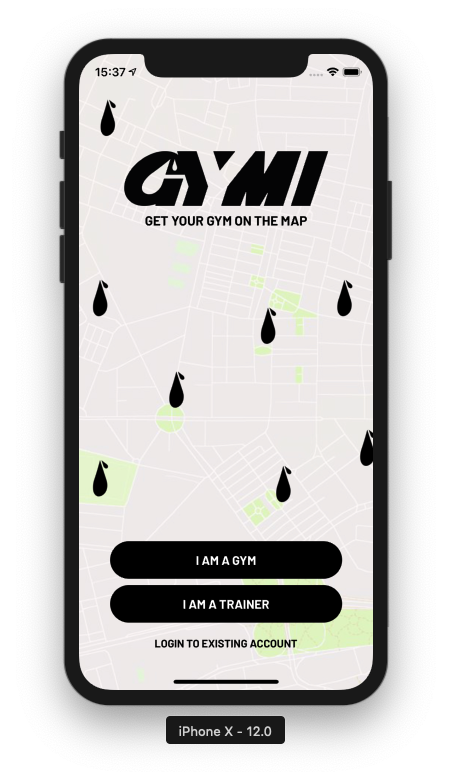
\includegraphics[width=0.4\textwidth]{pfc/figuras/landing.png}
    \caption{Tela de entrada do aplicativo}
    \label{fig:landing}
\end{figure}

% ******************
% Cadastro academias
% ******************
\subsection{Academias} \label{sec:register-gym}
Selecionada a opção por cadastro de um estabelecimento, o usuário primeiramente deve cadastrar os dados do administrador do local (ver Figura \ref{fig:register-manager-data}). Os seguintes dados são solicitados: primeiro nome, último nome, número do celular com código de área, e-mail (com campo de verificação) e senha (com campo de verificação). Para prosseguir com o cadastro, o usuário deve preencher os campos com dados válidos (caso contrário, alertas de erro são apresentados na tela). Ao clicar o botão "Next" uma chamada de API é feita ao back-end passando os dados digitados como parâmetro. Em caso de sucesso, a próxima tela do cadastro é apresentada; em caso de erro (como um e-mail de usuário já cadastrado), um alerta de erro é apresentado - Figura \ref{fig:register-manager-error}.

\begin{figure}[h]
	\centering
    \begin{subfigure}[b]{0.4\textwidth}
        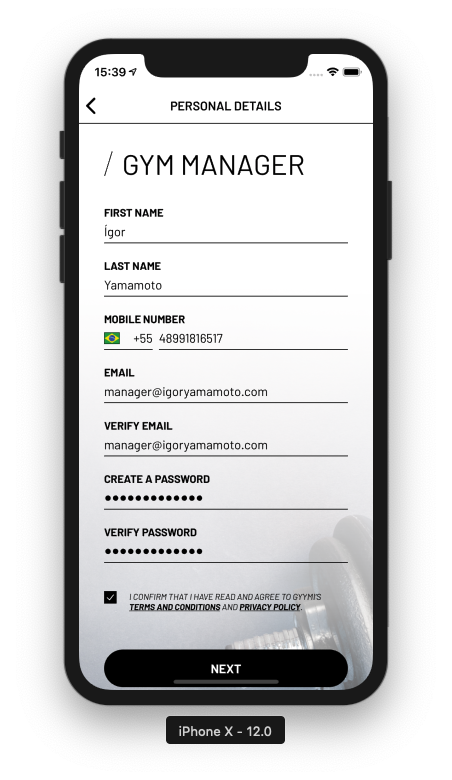
\includegraphics[width=\textwidth]{pfc/figuras/register-manager.png}
        \caption{Dados do administrador}
        \label{fig:register-manager-data}
    \end{subfigure}
    ~
	\begin{subfigure}[b]{0.4\textwidth}
        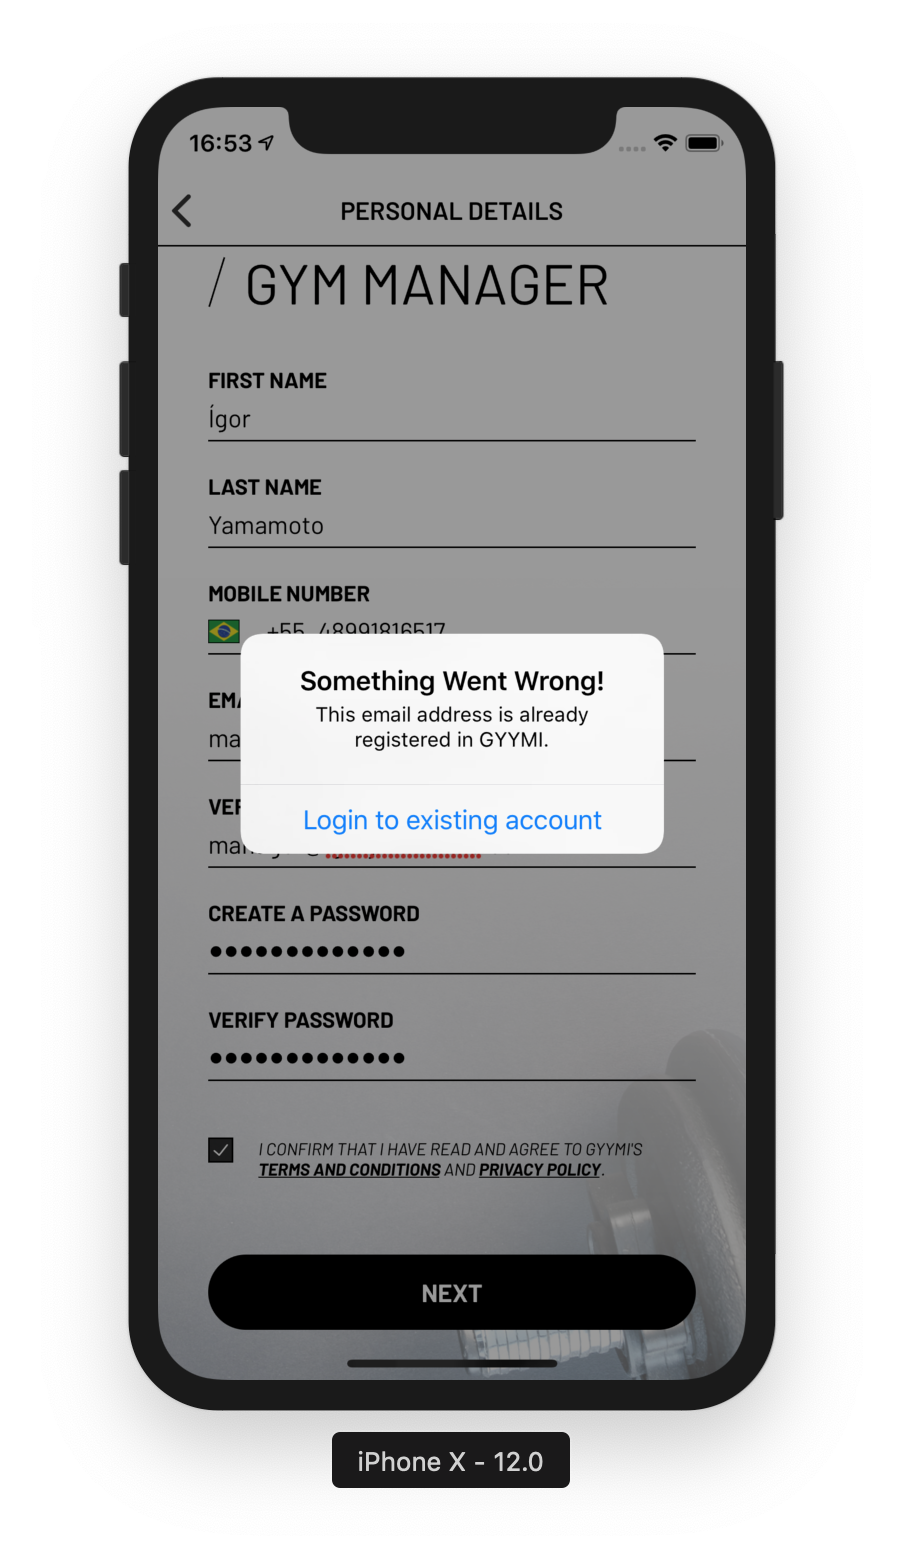
\includegraphics[width=\textwidth]{pfc/figuras/register-manager-error.png}
        \caption{Alerta de erro}
        \label{fig:register-manager-error}
    \end{subfigure}
    ~
    \caption{Tela de cadastro do usuário - administrador da academia}
    \label{fig:register-manager}
\end{figure}

Após o cadastro do usuário administrador da academia ter sido realizado com sucesso, o perfil do estabelecimento é cadastrado. Três telas fazem parte deste fluxo (ver Figura \ref{fig:register-gym}): primeiro informações gerais da academia (nome, endereço, número para contato com o estabelecimento, web-site e endereço de mídias sociais) devem ser passadas - Figura \ref{fig:register-gym-info}; em seguida um tela (Figura \ref{fig:register-gym-amenities}) com opções selecionáveis de facilidades e equipamentos fornecidos pela academia é apresentada; por último, o usuário tem a opção de carregar fotos do estabelecimento (Figura \ref{fig:register-gym-photos}), selecionando uma delas para ser exibida como foto de capa (a ser mostrada no perfil da academia).

\begin{figure}[H]
	\centering
    \begin{subfigure}[b]{0.3\textwidth}
        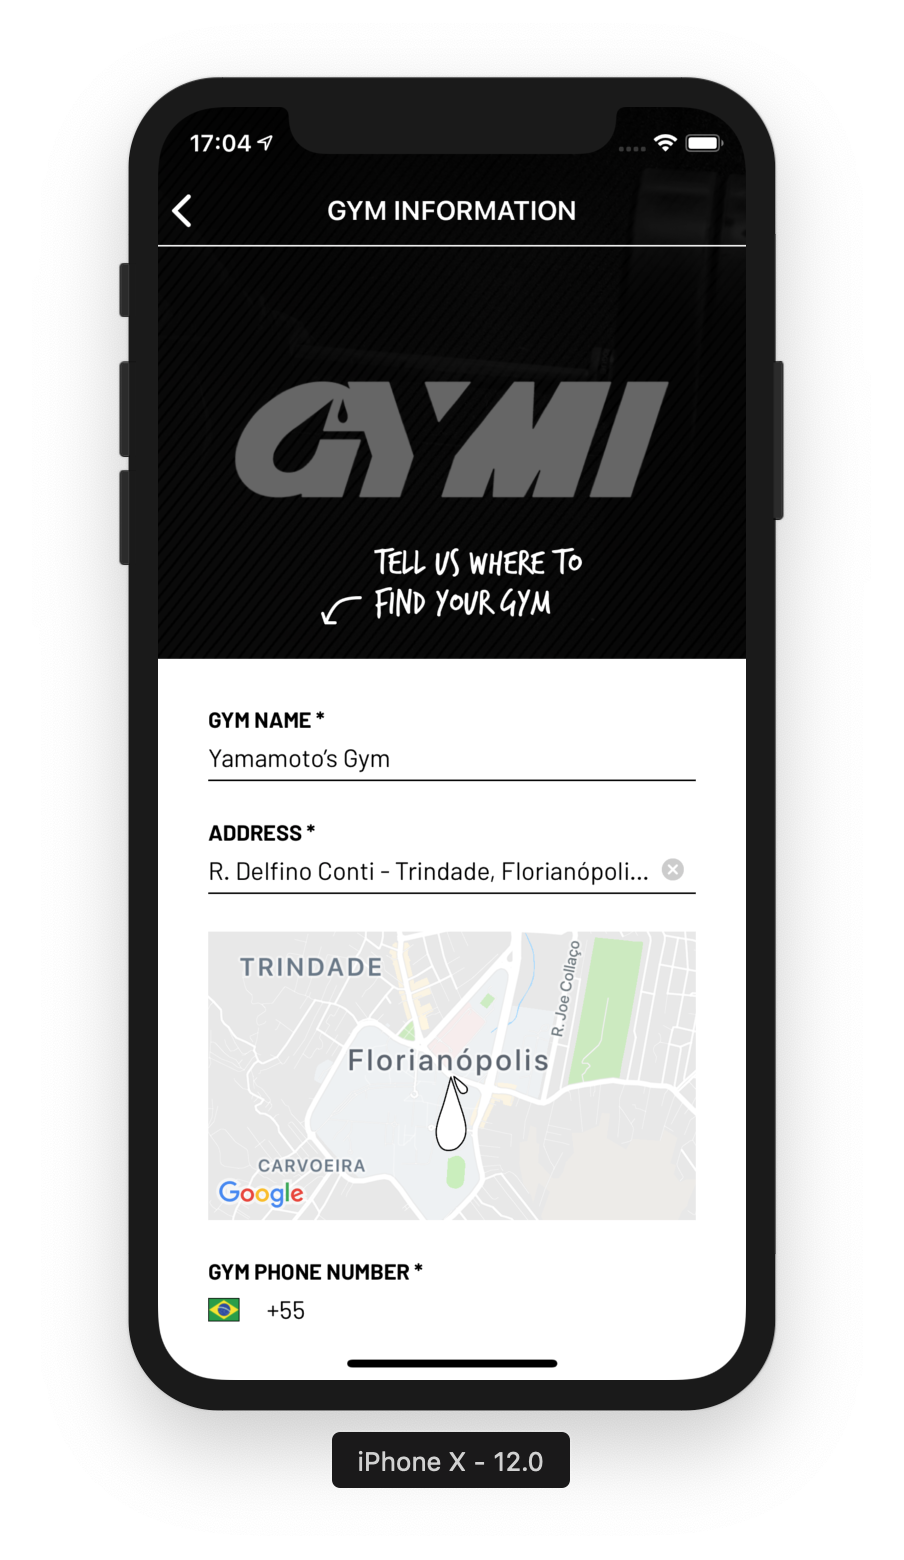
\includegraphics[width=\textwidth]{pfc/figuras/register-gym-info.png}
        \caption{Registro das informações gerais da academia}
        \label{fig:register-gym-info}
    \end{subfigure}
    ~
	\begin{subfigure}[b]{0.3\textwidth}
        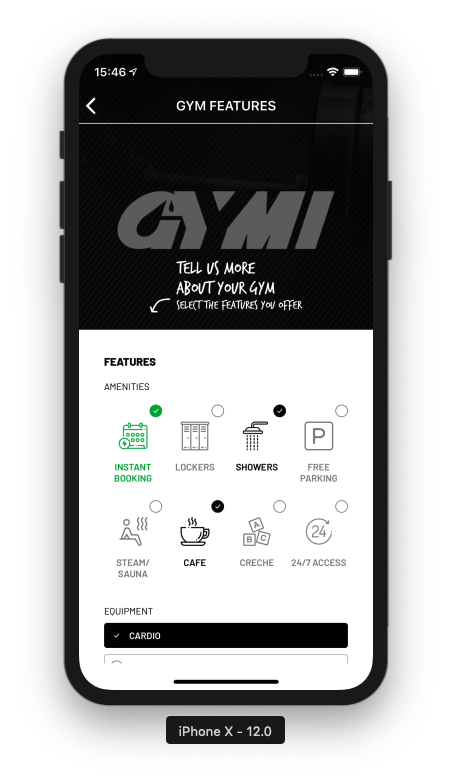
\includegraphics[width=\textwidth]{pfc/figuras/register-gym-amenities.png}
        \caption{Registro das facilidades e equipamentos}
        \label{fig:register-gym-amenities}
    \end{subfigure}
    ~
    \begin{subfigure}[b]{0.3\textwidth}
        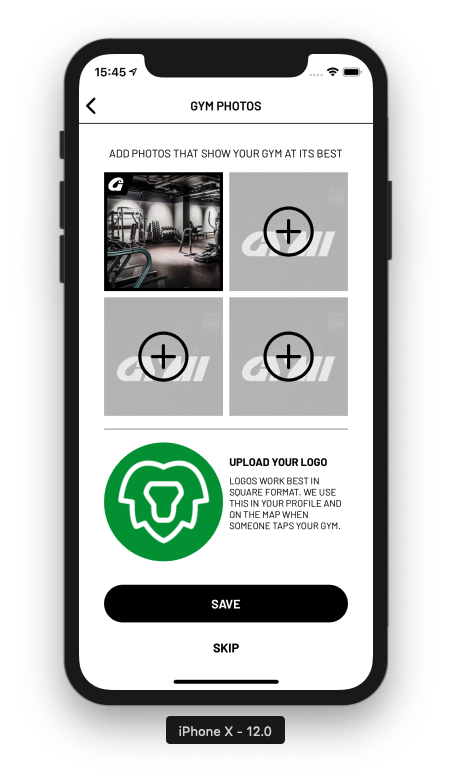
\includegraphics[width=\textwidth]{pfc/figuras/register-gym-photos.png}
        \caption{Registro das fotos do local e da logo}
        \label{fig:register-gym-photos}
    \end{subfigure}
    ~
    \caption{Telas de cadastro de um estabelecimento}
    \label{fig:register-gym}
\end{figure}

Ao término do cadastro do estabelecimento, uma tela de boas vindas (Figura \ref{fig:gym-welcome}) é apresentada ao usuário. A tela apresenta uma marcação (gota de suor branca) da academia em um mapa no local real cadastrado anteriormente (mapa obtido através do serviço do sistema de geolocalização, que é apresentado no próximo capítulo) e outros locais já cadastrados na plataforma são demarcados também (gotas pretas de suor menores), informação proveniente do back-end. A tela apresenta duas opções de ação: registrar detalhes da conta bancária (opção "Add bank details", tela não implementada para a versão piloto do aplicativo) e uma opção para pular o cadastro da conta (opção "Skip"). Ambas as ações levam o usuário as telas de uso da academia, que são apresentadas nas próximas secções.

\begin{figure}[ht]
    \centering
    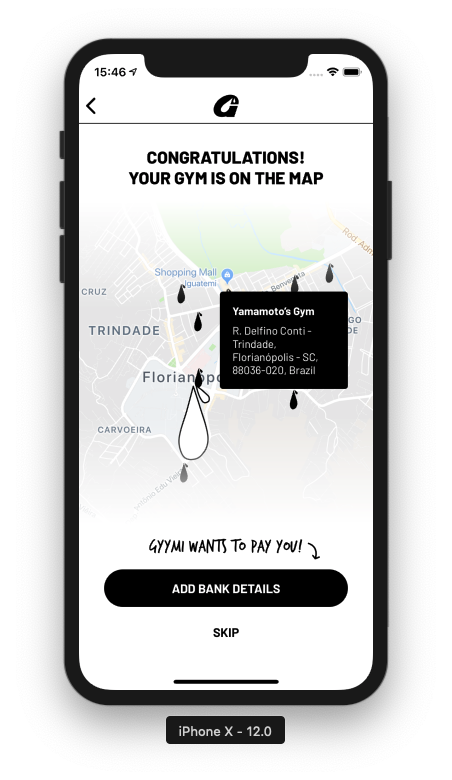
\includegraphics[width=0.4\textwidth]{pfc/figuras/gym-welcome.png}
    \caption{Tela de boas vindas para o estabelecimento}
    \label{fig:gym-welcome}
\end{figure}

% ********************
% Cadastro Treinadores
% ********************
\subsection{Treinadores}
Caso o usuário selecione a opção de cadastro de um treinador na tela de entrada, o mesmo é redirecionado para a tela de cadastro de informações gerais de usuário (Figura \ref{fig:register-trainer-info}), com os seguintes campos de dados: primeiro nome, último nome, e-mail, número do celular, senha (com campo de verificação). Caso as informações preenchidas sejam válidas, o cadastro prossegue para a próxima tela; caso contrário, alertas de erros são exibidos (como no caso do estabelecimento - Secção \ref{sec:register-gym})

Após o preenchimento dos campos, uma requisição para registrar os dados na plataforma é feita para o back-end, o qual faz uma requisição ao serviço de envio de SMS com os dados do número do celular do usuário. Este serviço então envia um SMS com um código de verificação, que deve ser preenchido no campo "Verification Code" da tela de verificação por SMS (ver Figura \ref{fig:register-trainer-verification}). Nesta tela o usuário tem duas opções de ação: verificar o código preenchido (opção que dispara uma nova requisição ao back-end para identificar se o código fornecido é o mesmo gerado pelo serviço de SMS) ou reenviar o código de verificação (opção que desencadeia um novo envio de SMS para o usuário através de nova solicitação para tal ao serviço de SMS).

\begin{figure}[h]
	\centering
    \begin{subfigure}[b]{0.4\textwidth}
        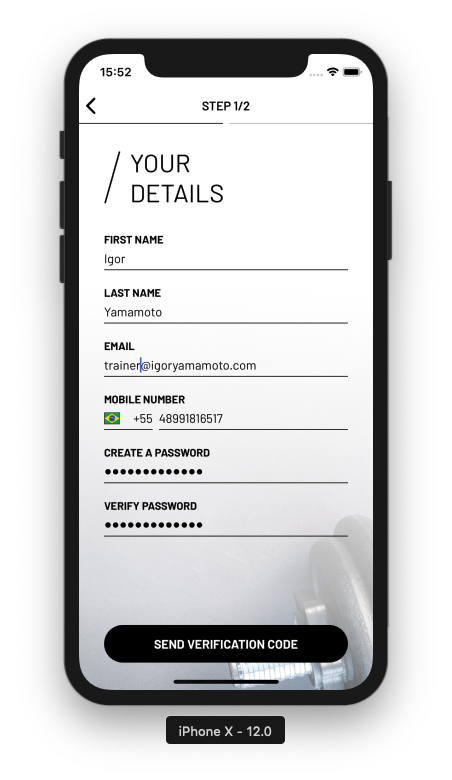
\includegraphics[width=\textwidth]{pfc/figuras/register-trainer.png}
        \caption{Dados do treinador}
        \label{fig:register-trainer-info}
    \end{subfigure}
    ~
	\begin{subfigure}[b]{0.4\textwidth}
        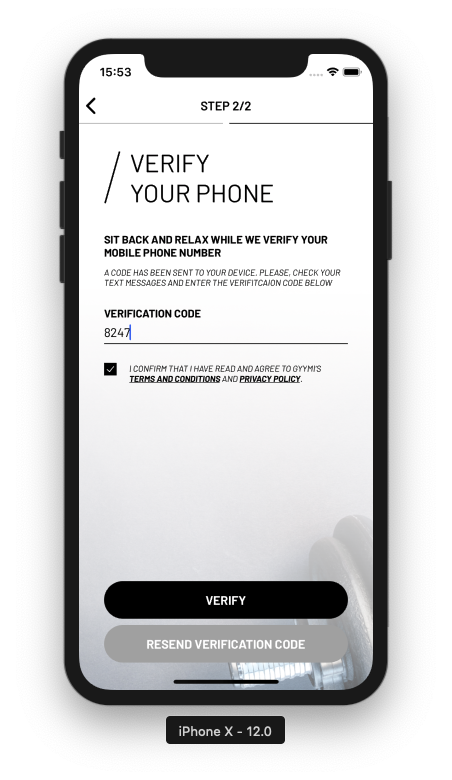
\includegraphics[width=\textwidth]{pfc/figuras/register-trainer-verification.png}
        \caption{Verificação por SMS}
        \label{fig:register-trainer-verification}
    \end{subfigure}
    ~
    \caption{Tela de cadastro do usuário - treinador pessoal}
    \label{fig:register-trainer}
\end{figure}

Uma vez que o código de verificação é validado, o fluxo prossegue para uma tela de boas vindas (Figura \ref{fig:tr-welcome}). Nesta tela, o usuário tem a ação de configurar seu perfil de treinador (opção "Set up your trainer profile") ou a ação de pular esta etapa (opção "Skip"). Caso selecionada a opção de configuração, o cadastro prossegue; caso selecionada a outra opção, o usuário é direcionado a tela principal do treinador.

\begin{figure}[h]
    \centering
    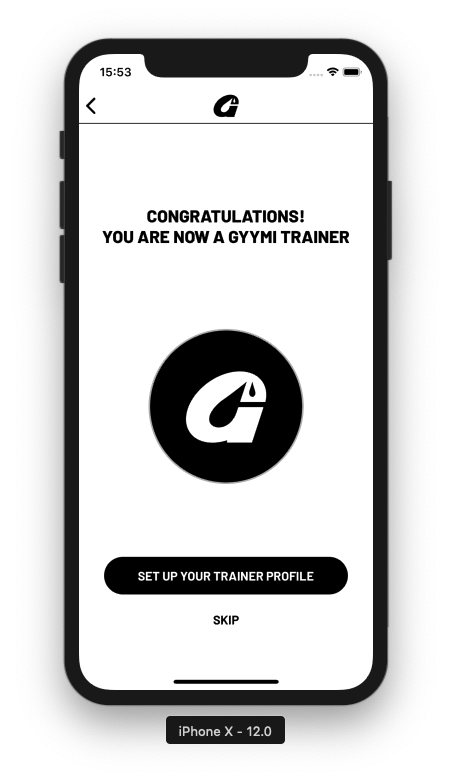
\includegraphics[width=0.4\textwidth]{pfc/figuras/tr-congratulations.png}
    \caption{Tela de boas vindas para o treinador}
    \label{fig:tr-welcome}
\end{figure}

A configuração de perfil de treinador segue um fluxo de três telas (Figura \ref{fig:register-tr-profile}). Primeiro, o usuário deve registrar as informações gerais do perfil (Figura \ref{fig:register-tr-profile-info}), informando de forma opcional os campos: mantra, área de treino, endereço de mídias sociais e web-site. Em seguida, o usuário é direcionado a uma tela com opções selecionáveis de habilidades e especialidades (Figura \ref{fig:register-tr-skills}) que ele pode oferecer em seus treinos físicos. Por último, uma tela de confirmação do cadastro do perfil é exibida (Figura \ref{fig:register-tr-profile-confirmation}), com opções de edição caso o usuário deseje alterar alguma informação. Ao pressionar o botão de confirmar, uma requisição é feita ao back-end passando os dados de perfil do treinador para registro no sistema. Após a requisição ter obtido sucesso, o usuário é direcionado a tela principal de uso do aplicativo do treinador, a ser apresentada nas próximas secções.

\begin{figure}[H]
	\centering
    \begin{subfigure}[b]{0.3\textwidth}
        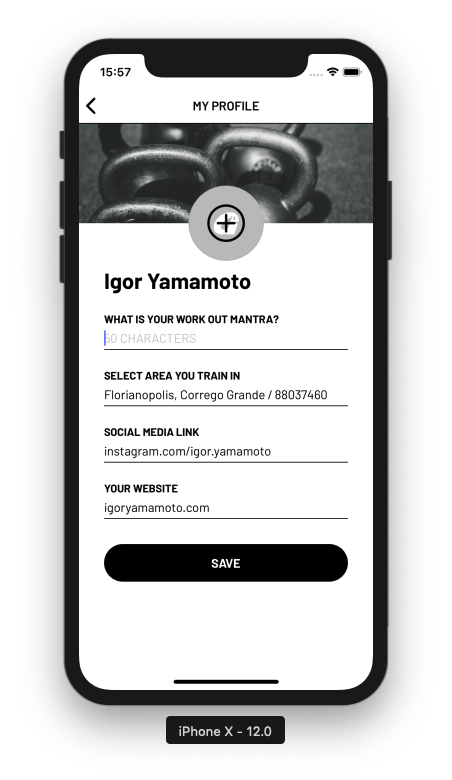
\includegraphics[width=\textwidth]{pfc/figuras/tr-register-profile-1.png}
        \caption{Registro das informações gerais do treinador}
        \label{fig:register-tr-profile-info}
    \end{subfigure}
    ~
	\begin{subfigure}[b]{0.3\textwidth}
        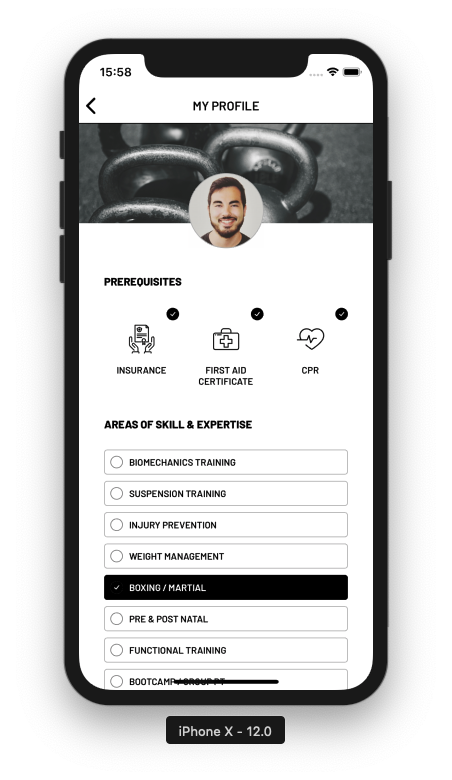
\includegraphics[width=\textwidth]{pfc/figuras/tr-register-profile-2.png}
        \caption{Registro das habilidades e especialidades}
        \label{fig:register-tr-skills}
    \end{subfigure}
    ~
    \begin{subfigure}[b]{0.3\textwidth}
        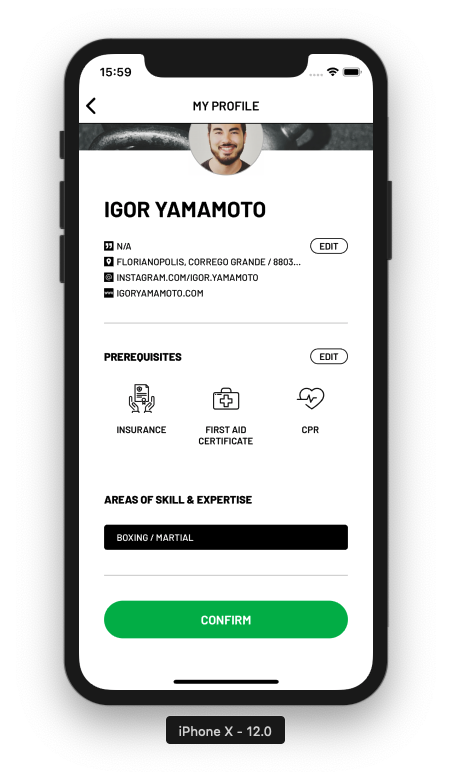
\includegraphics[width=\textwidth]{pfc/figuras/tr-register-profile-3.png}
        \caption{Confirmação do registro de perfil}
        \label{fig:register-tr-profile-confirmation}
    \end{subfigure}
    ~
    \caption{Fluxo de cadastro de perfil de treinador}
    \label{fig:register-tr-profile}
\end{figure}

% *******************
% Interface academias
% *******************
\section{Interface para Academias}
Nesta secção, é apresentada a interface de uso dos usuários que cadastraram um estabelecimento na plataforma. As principais funcionalidades implementadas para a versão piloto do aplicativo são abordadas: dashboard com dados semanais de uso da academia, calendário de sessões agendadas e configuração de agenda semanal para locação, perfil da academia.

Na interface para as academias o usuário tem a opção de navegar por cinco telas principais, selecionadas a partir da barra de navegação na parte inferior do aplicativo (Figura \ref{fig:gym-tabbar}). Da esquerda para a direita, as opções de navegação são: dashboard da academia; treinadores com sessões agendadas (não implementado para o piloto); calendário de sessões agendadas; central de notificações (não implementado para o piloto); perfil do estabelecimento.

\begin{figure}[h]
    \centering
    
\includegraphics{pfc/figuras/gym-tabbar.png}
    \caption{Barra de navegação da interface para academias}
    \label{fig:gym-tabbar}
\end{figure}


\subsection{Dashboard da Academia}
A tela de dashboard da academia (Figura \ref{fig:gym-dashboard}) apresenta dados de uso e de receita semanais do estabelecimento. Os dados são baseados nos agendamentos realizados pelos treinadores e são provenientes de uma chamada de API feita ao back-end, que realiza a lógica do cálculo a partir das informações armazenadas no banco de dados da plataforma. Os seguintes dados da semana atual e passada são apresentados no painel: receita total, número total de agendamentos, número total de treinadores, número total de hora agendadas por treinadores.

\begin{figure}[H]
    \centering
    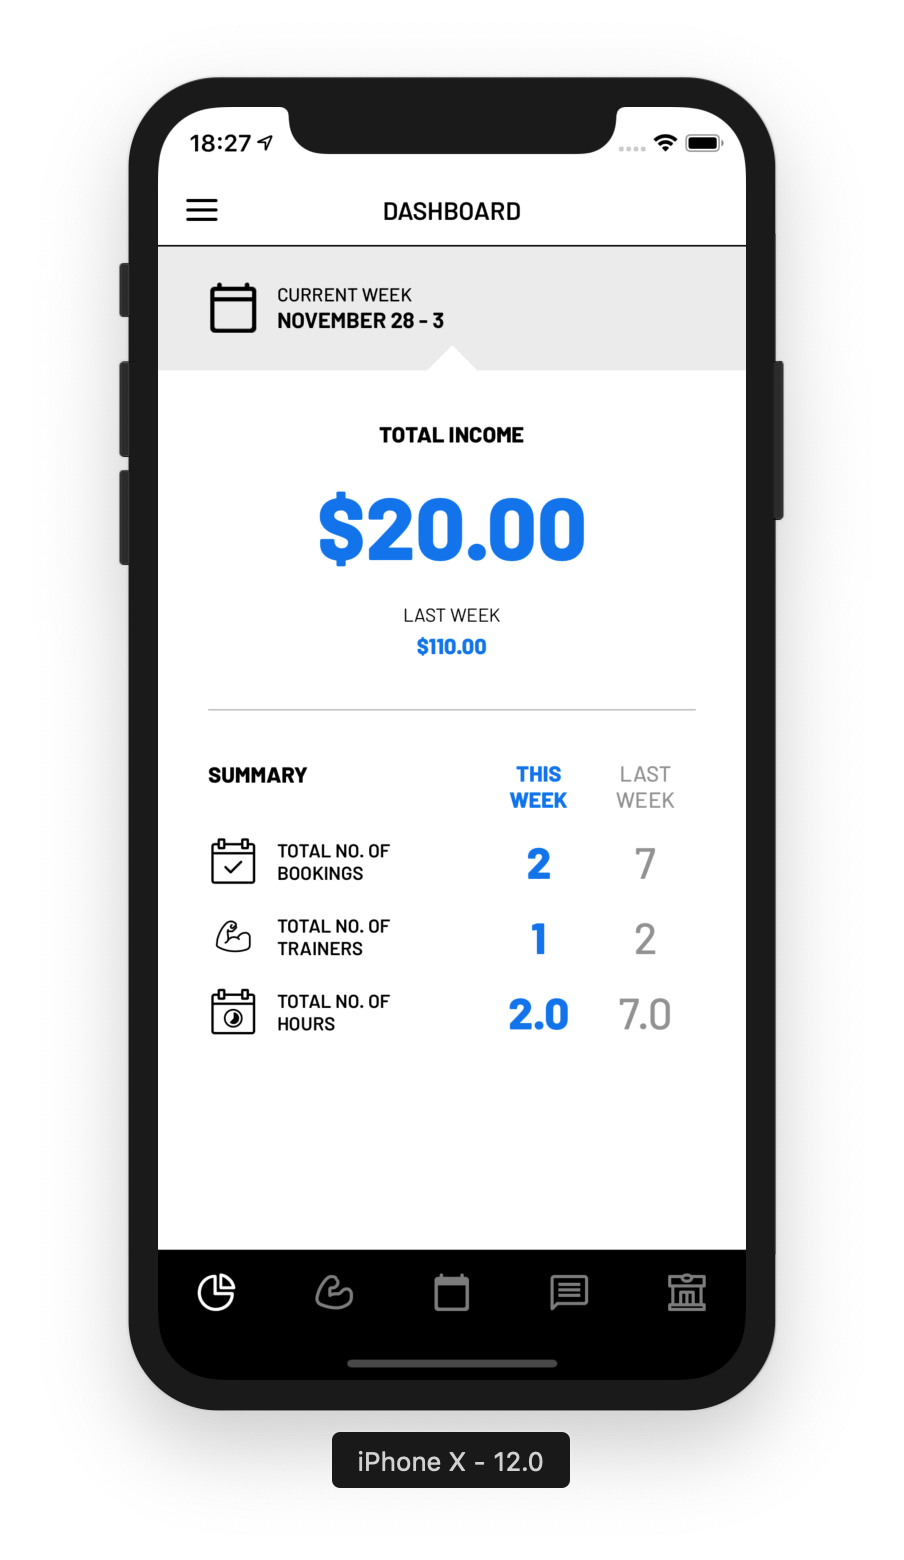
\includegraphics[width=0.4\textwidth]{pfc/figuras/gym-dashboard.png}
    \caption{Tela de dashboard da academia}
    \label{fig:gym-dashboard}
\end{figure}

\subsection{Agenda para Locação}

\begin{figure}
    \centering
    \includegraphics{}
    \caption{Caption}
    \label{fig:my_label}
\end{figure}

\subsection{Calendário de Sessões Agendadas}

\subsection{Perfil do Estabelecimento}


% *********************
% Interface treinadores
% *********************
\section{Interface para Treinadores}

\subsection{Perfil do Treinador}

\subsection{Busca por Academias}

\subsection{Agendamento de Sessão}

\subsection{Calendário de Sessões Agendadas}
